\documentclass[herrin-thesis.tex]{subfiles}
\begin{document}

\chapter{Measuring Double-beta Decay}
\label{ch:analysis}

\section{Event Selection}
\subsection{Timing-based Vetoes}
In order to reduce backgrounds (described in \cref{sec:muon_motivation}) due to cosmic-ray muons, two cuts are applied to the data:
\begin{itemize}
\item Events that occur within the \SI{25}{\ms} following a hit in a muon veto system panel are cut.
\item Events that occur within the \SI{60}{\s} following a muon passing through the TPC (identified by the method in \cref{ch:muons}) are cut. The muon events are cut themselves, as well.
\end{itemize}
These cuts are designed to remove as many cosmogenic background events as possible while not cutting a portion of the detector live time so large that the trade-off in signal-to-background ratio is not worth it.

Events occurring near each other in time are likely to be due to a decay of some radioactive contaminant, followed by another decay of a short-lived daughter. For example, the \isotope{222}{Rn} daughter \isotope{214}{Bi} \(\beta^{-}\) decays to \isotope{214}{Po}, which then \(\alpha\) decays with a \SI{164}{\micro\s} half-life.  Any event is vetoed if it occurs within \SI{\pm1}{\s} of another event.

Finally, conditions external to the detector may make the data unusable. Data from these time periods is vetoed.The most common cause is the mine evacuation siren, which is tested periodically. It is loud enough to create a large amount electronic noise through microphonic pickup. Time periods in which the siren is going off are vetoed.

The effects of all timing-based vetoes are summarized in \cref{tab:analysis_veto_effects}.

\begin{table}[htb]
\centering
\caption[Impact of timing-based vetoes]{A breakdown of the impact of the muon vetoes, TPC event-event coincidence vetoes, and the external conditions vetoes on the detector live time. Since multiple vetoes can be in effect at the same time, the combined impact of some vetoes is not simply their sum.}
\label{tab:analysis_veto_effects}
\begin{tabular}{l l l l c c}\toprule
\multicolumn{4}{c}{}							&	Time (\si{hr})	&	\%	\\\midrule
\multicolumn{4}{l}{Vetoed Time}				&	400.2		&	12.5	\\
	&\multicolumn{3}{l}{External Conditions}		&	18.4			&	0.6	\\
	&\multicolumn{3}{l}{Physics Vetoes}			&	381.8		&	11.9	\\
	&&\multicolumn{2}{l}{Muons}				&	163.5		&	5.1	\\
	&&&TPC Muon							&	144.8		&	4.5	\\
	&&&Panel Muon						&	19.6			&	0.6	\\
	&&\multicolumn{2}{l}{Event-Event Coincidence}&	236.5		&	7.4	\\
\multicolumn{4}{l}{Live Time}					&	2796.1		&	87.5	\\\midrule
\multicolumn{4}{l}{Total}						&	3196.3		&	100.0\\\bottomrule
\end{tabular}
\end{table}

\subsection{Other Vetoes}
\subsubsection{Scintillation-to-ionization ratio}
As mentioned in \cref{sec:xe_combining_ion_and_scint}, \(\alpha\) particle interactions produce more scintillation and less ionization in the liquid xenon than \(\beta\) and \(\gamma\) interactions. Therefore, events with a large scintillation-to-ionization ratio are removed from the data used for double beta decay physics. Since \isotope{222}{Rn} is a common source of \(\alpha\) particles, these decays are later used in order to constrain backgrounds due to other isotopes in the \isotope{222}{Rn} decay chain.

\subsubsection{Scintillation Timing}
Events are vetoed if they contain more than one scintillation cluster. The typical event rate in the TPC is \about{}\SI{0.1}{\Hz}, so random coincidences are rare enough that the effects of this cut on legitimate events is minuscule compared to other sources of systematic error. This eliminates \isotope{214}{Bi}-\isotope{214}{Po} coincidences, as described above, and also eliminates events in which there could be ambiguity in associating ionization signals with multiple scintillation signals. Additionally, events are vetoed if the scintillation comes too late in the waveform form ionization to have time to drift the full TPC drift length. Since the waveforms are centered around the trigger time, this does not happen in typical data, but may happen in source calibration runs.

\subsection{Fiducial Volume}
\label{sec:analysis_fiducial_volume}
\begin{figure}[htb]
\centering
	\begin{subfigure}[b]{0.48\textwidth}
	\centering
	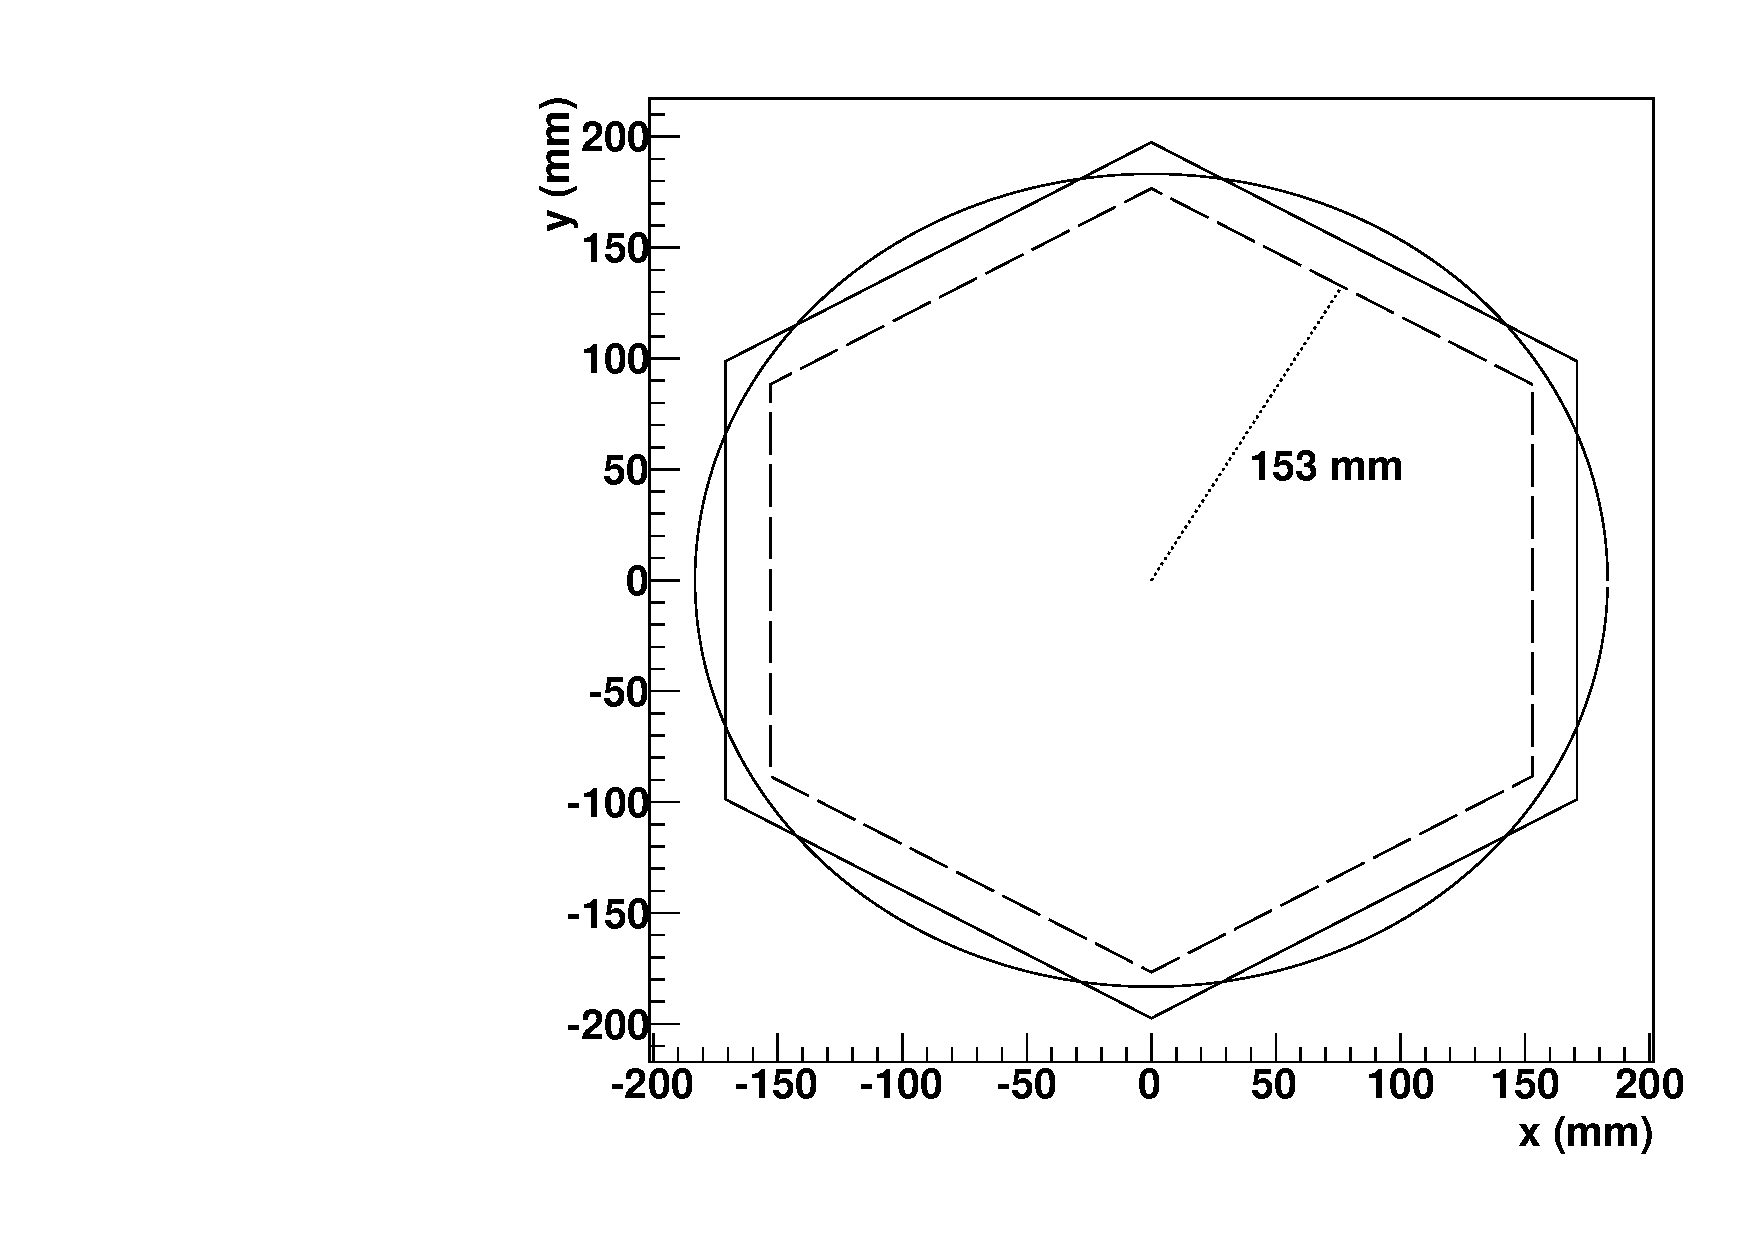
\includegraphics[width=\textwidth]{./plots/analysis_fiducial_vol_xy.pdf}
\end{subfigure}\hfill%
\begin{subfigure}[b]{0.48\textwidth}
	\centering
	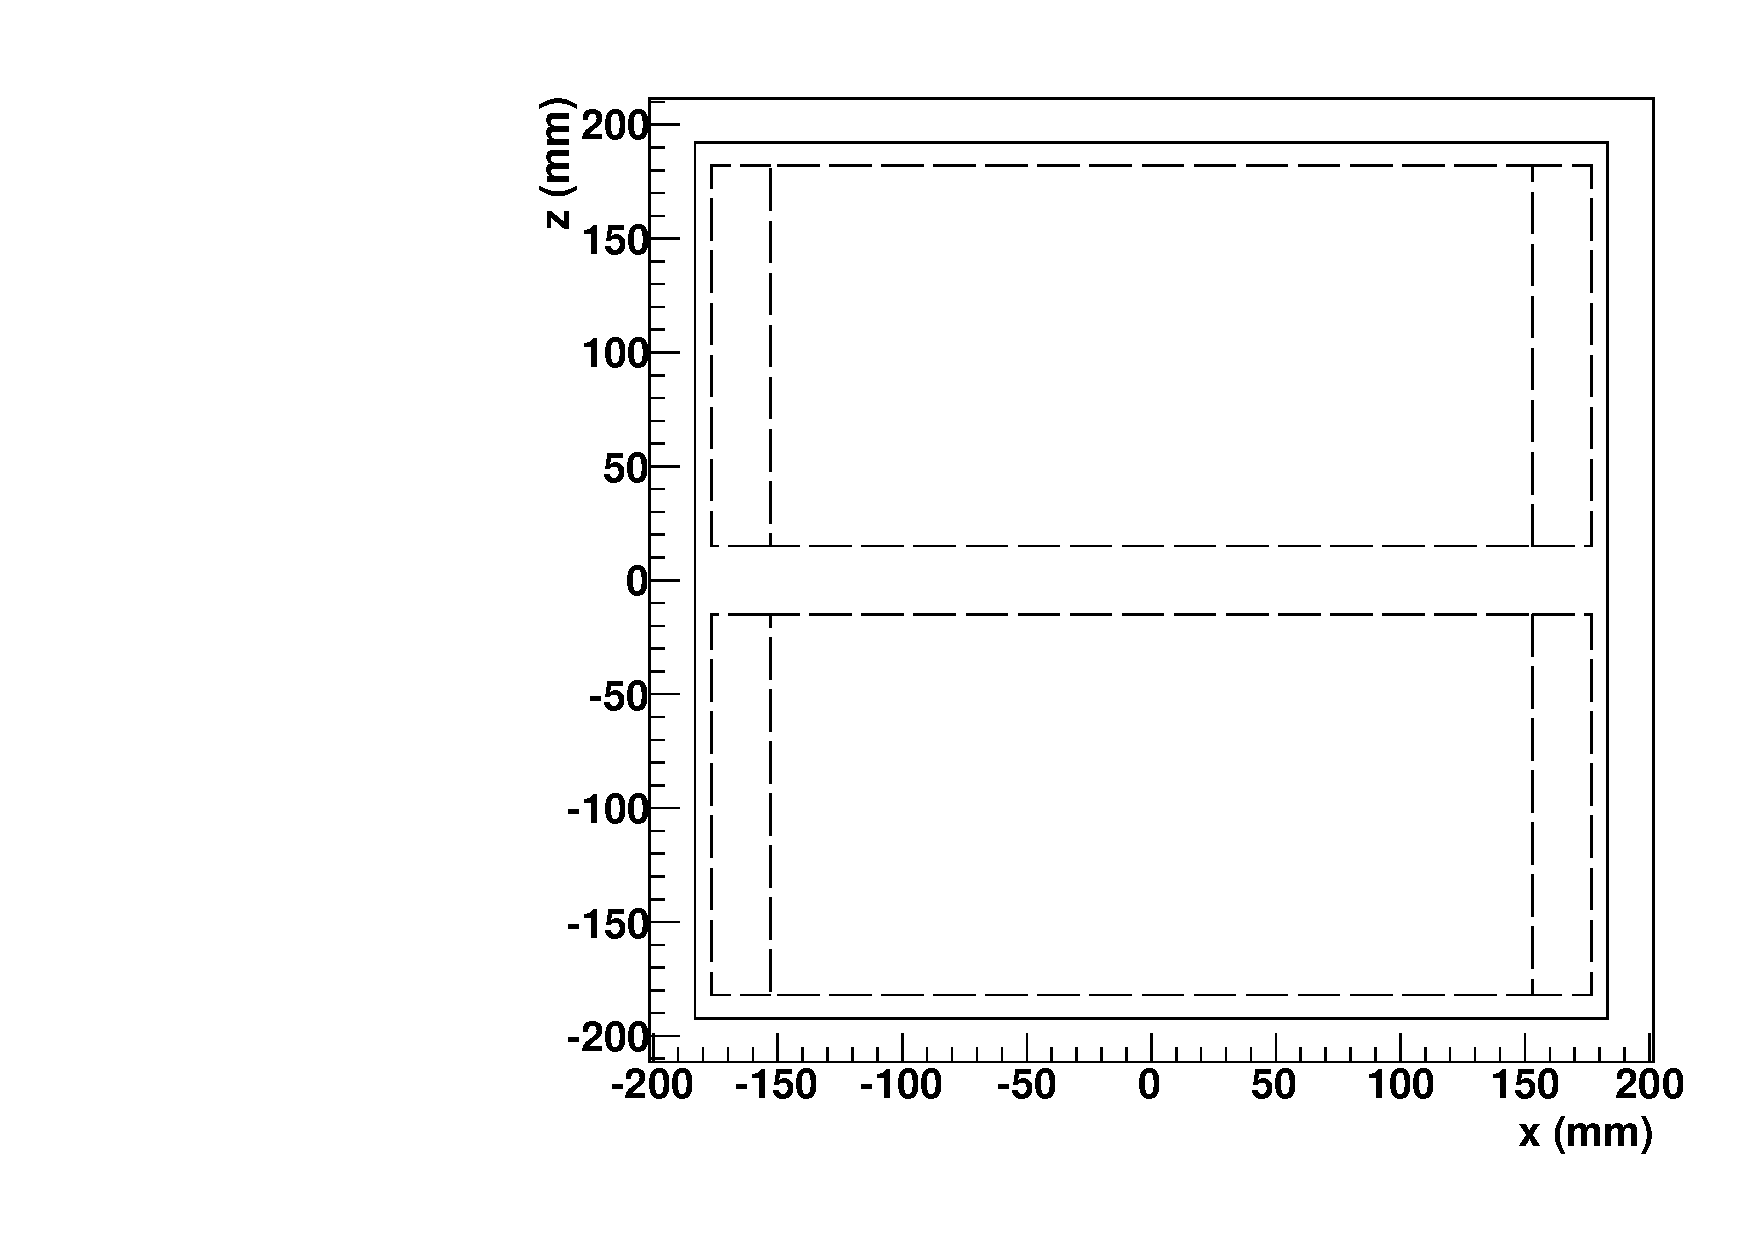
\includegraphics[width=1\textwidth]{./plots/analysis_fiducial_vol_xz.pdf}
	\end{subfigure}
\caption[Fiducial Volume]{Projections of the hexagonal fiducial volume. The dashed lines represent the fiducial volume. The solid lines are the anode wire plane and the teflon reflector. For the \(xz\) projection on the right, the two sets of vertical dashed lines are the maximum and minimum radial boundaries of the fiducial volume.}
\label{fig:analysis_fiducial_volume}
\end{figure}

All the liquid xenon within the teflon reflectors and between the anodes is ``active''. That is, ionization and scintillation in the active region are collected. However, only events within a fiducial volume are used in the analysis. This fiducial volume is a right hexagonal prism. The hexagon is coaxial with the detector and has apothem \SI{153}{\mm}. In each TPC, it begins \SI{5}{\mm} away from the cathode and extends to \SI{182}{\mm} (which is \SI{10.2}{\mm} from the \(v\) wire plane). \Cref{fig:analysis_fiducial_volume} provides an illustration. The total volume is \SI{27.1}{\litre}, which contains \SI{81.9}{\kg} of liquid xenon.

\begin{figure}[htb]
\centering
	\begin{subfigure}[b]{0.48\textwidth}
	\centering
	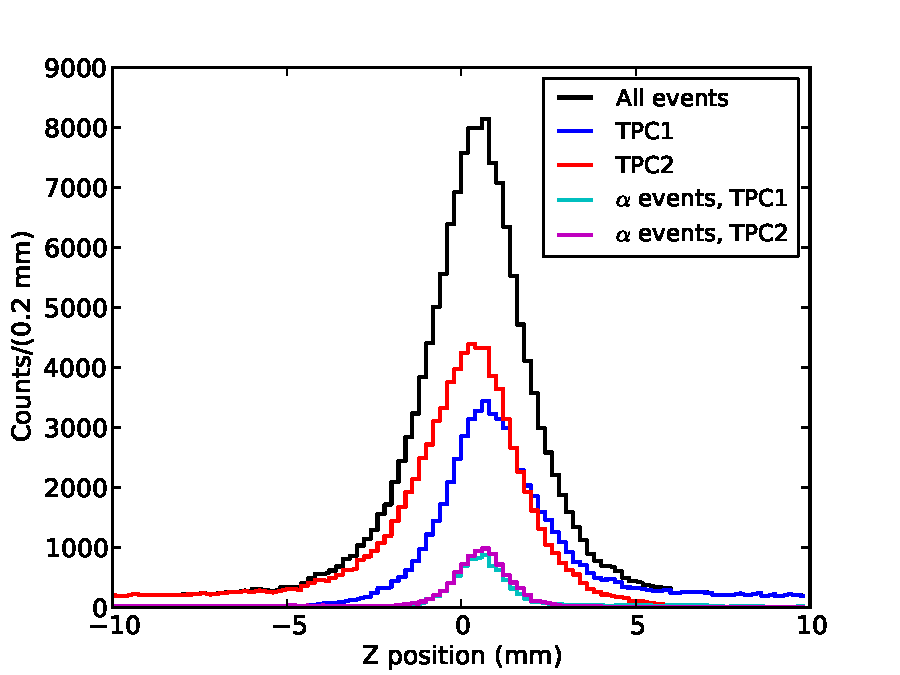
\includegraphics[width=\textwidth]{./plots/analysis_fiducial_vol_bg_cathode.pdf}
\end{subfigure}\hfill%
\begin{subfigure}[b]{0.48\textwidth}
	\centering
	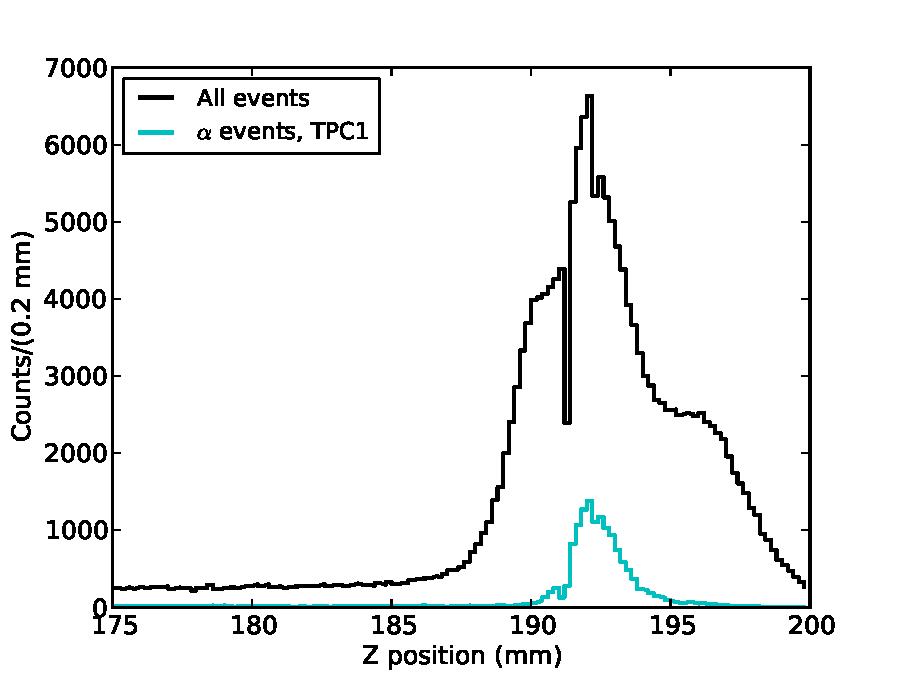
\includegraphics[width=1\textwidth]{./plots/analysis_fiducial_vol_bg_anode.pdf}
	\end{subfigure}
\caption[Increased event rates near cathode and anodes]{The choice of fiducial volume is partially motivated by the increased event rate seen near the cathode (at \(z = \SI{0}{\mm}\)) (shown left) and near the anodes (shown right; the \(v\) plane is at \(|z|=\SI{192}{\mm}\) and the \(u\) plane is at \(|z|=\SI{198}{\mm}\)). An increase is seen for both the total event rate, and for the rate of \(\alpha\) particle interactions, which suggests the increased rate is due to backgrounds. Requiring \(\SI{5}{\mm} < |z| < \SI{182}{\mm}\) puts the fiducial volume well away from the volumes that show an increased rate.}
\label{fig:analysis_fiducial_vol_bg_rates}
\end{figure}

This particular choice of fiducial volume has two chief motivations. The first is to reduce radioactive backgrounds from the detector materials. \Cref{fig:analysis_fiducial_vol_bg_rates} shows event rates near the cathode and anodes. There is nothing special about the xenon near these planes, and so the increased event rate must be due to backgrounds. The \(z\) cuts above eliminate the volumes that show higher-than-typical event rates.

\begin{figure}[htb]
\centering
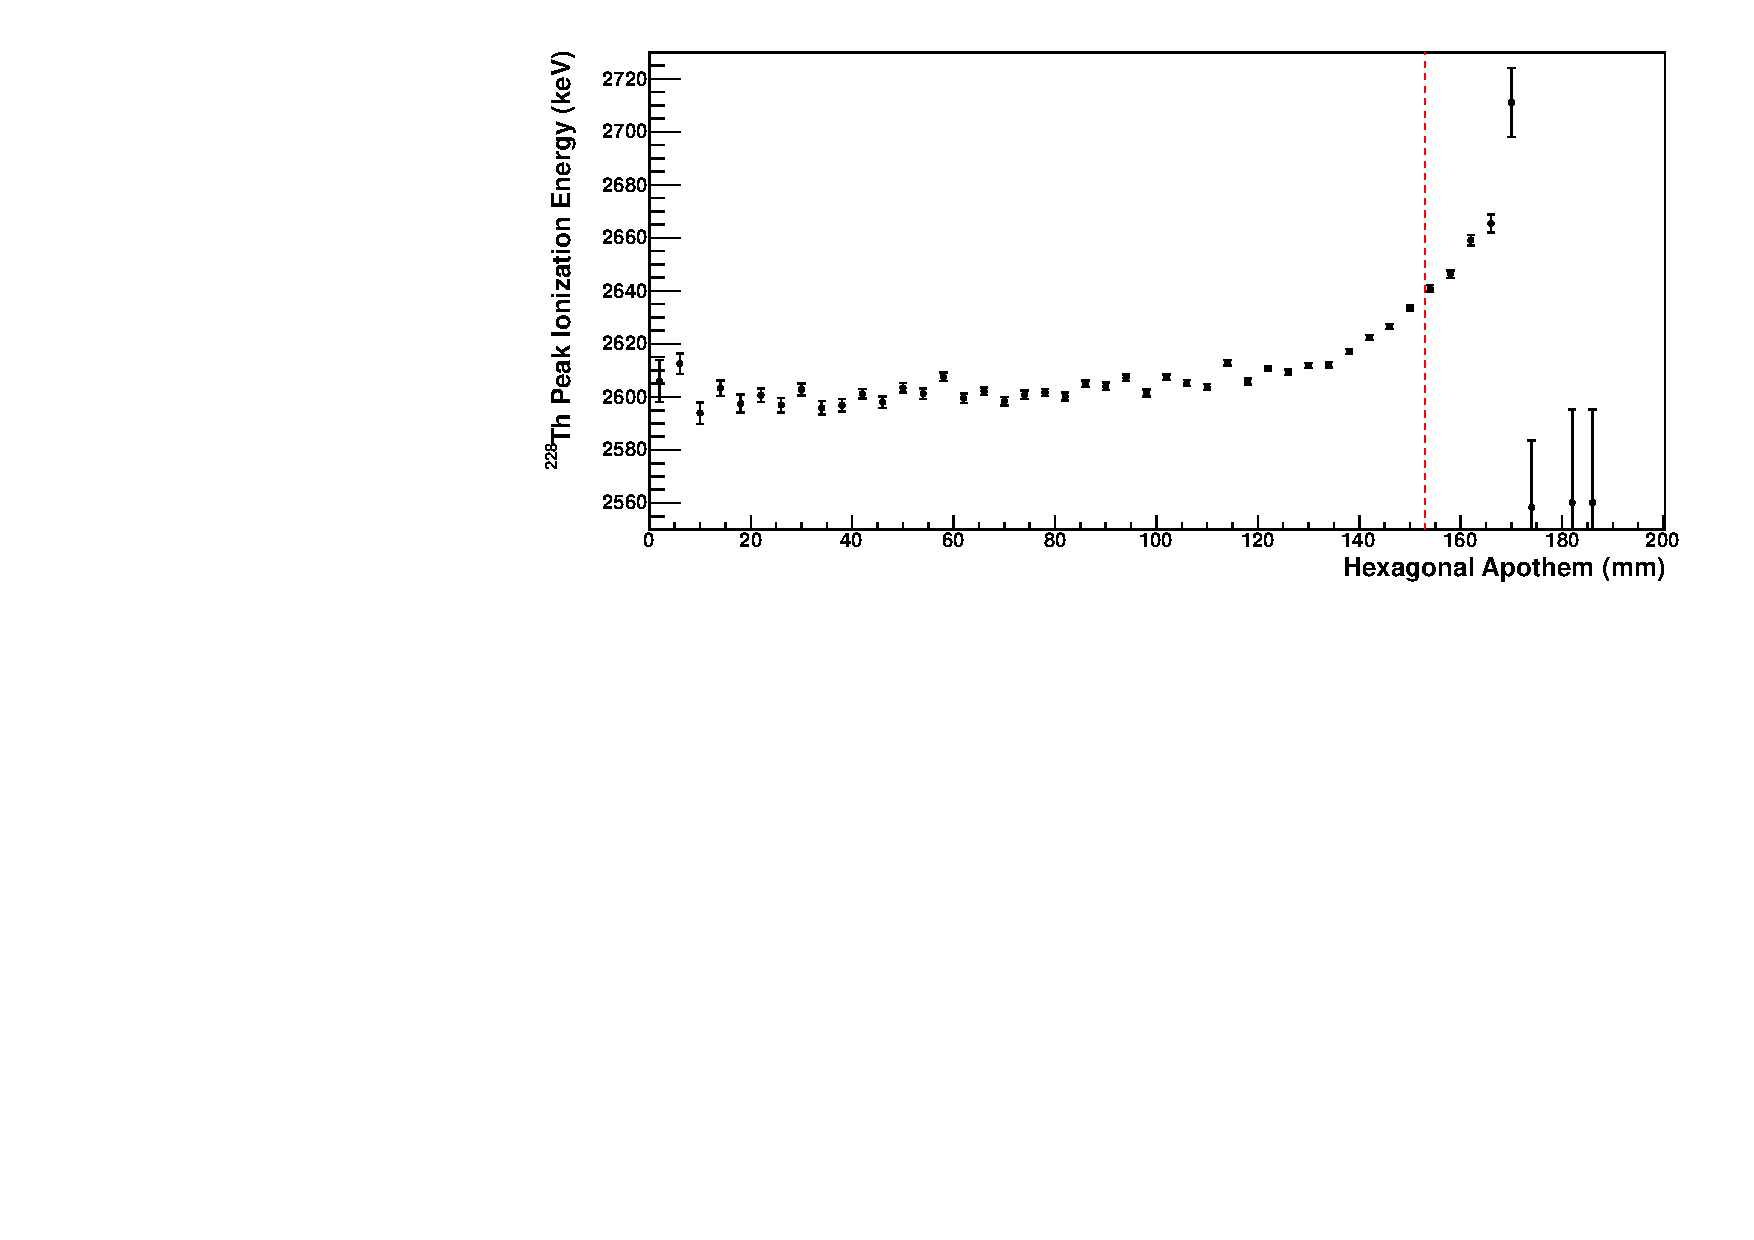
\includegraphics[width=0.8\textwidth]{./plots/analysis_fiducial_vol_transverse.pdf}
\caption[Energy response due to increasing fiducial volume apothem]{The reconstructed energy of the \SI{2615}{\keV} peak from a \isotope{228}{Th} source calibration. This is found by fitting a Gaussian + complimentary error function model to data with an increasingly large allowed fiducial volume. A larger allowed hexagonal apothem extends the fiducial volume closer and closer to the edges of the anode wire planes. The detector response begins to deviate significantly when the cut is extended above \SI{153}{\mm}, and so this is used to define the fiducial volume.}
\label{fig:analysis_fiducial_vol_bg_rates}
\end{figure}

The second motivation is to ensure a homogeneous detector response inside the fiducial volume. As shown in the previous discussion of the shielding grid correction in \cref{sec:data_grid_correction}, the correction becomes significant near \(|z|=\SI{182}{\mm}\) (see \cref{fig:data_grid_correction_fits}). Even with the correction applied, the detector response begins to diverge near that position (see \cref{fig:data_grid_correction_applied}), and so it is used as the boundary of the fiducial region. In the transverse dimension, a hexagonal cross-section is used. This matches the anode wire geometry, and so makes applying the fiducial volume cut straightforward. \Cref{fig:analysis_fiducial_vol_transverse} shows that requiring the apothem of this hexagon to be less than \SI{153}{\mm} ensures uniform energy response.

\subsection{Quantities of Interest}
Once an event passes the data quality cuts, the following quantities are calculated:
\begin{enumerate}
\item The multiplicity (single site or multiple site), using the criteria described in \cref{sec:data_topology}.
\item The event energy using the calibration obtained as described in \cref{sec:data_calibration}.
\item The ``standoff distance''. The radial distance of the cluster to the teflon reflector is calculated. So is the \(z\) distance to the \(v\) wire plane. The standoff distance is the minimum of these two distances.
\end{enumerate}

The singles site and multiple site information helps separate \(\gamma\) interactions from \(\beta\) interactions. The standoff distance describes the spatial distribution of events. For example, the distribution of \twonu{} events, since they are uniformly distributed in the detector, have a standoff distance distribution that extends to higher values. The distribution of background events from detector materials, on the other hand, peaks at small standoff distances. And, of course, the energy spectra of different types of decay are different.

\section{Monte Carlo Simulations of Signals and Backgrounds}
\subsection{PDF Generation}

The GEANT4 simulation toolkit\cite{Agostinelli:2003fk} is used in order to determine both the energy spectra and spatial distributions of various double beta decay signals and radioactive backgrounds in EXO-200.

All double beta decay modes are simulated using the Fermi function by Schenter and Vogel\cite{Schenter:1983uq}.

\section{Systematic Uncertainties}

\section{Maximum Likelihood Method}

\section{Measurement of \twonu}

\subsection{Consistency Checks}

\section{Limits on \(0\nu\beta\beta\chi^0(\chi^0)\)}

\end{document}
